%%% template.tex
%%%
%%% This LaTeX source document can be used as the basis for your technical
%%% paper or abstract. Intentionally stripped of annotation, the parameters
%%% and commands should be adjusted for your particular paper - title, 
%%% author, article DOI, etc.
%%% The accompanying ``template.annotated.tex'' provides copious annotation
%%% for the commands and parameters found in the source document. (The code
%%% is identical in ``template.tex'' and ``template.annotated.tex.'')

\documentclass[conference]{acmsiggraph}
\usepackage{subcaption}
\TOGonlineid{45678}
\TOGvolume{0}
\TOGnumber{0}
\TOGarticleDOI{1111111.2222222}
\TOGprojectURL{}
\TOGvideoURL{}
\TOGdataURL{}
\TOGcodeURL{}

\title{A Triangle Mesh Approach to Painting}

\author{Mark D. Benjamin\thanks{e-mail:mdbenjam@princeton.edu} \hspace{10 pt} Princeton Unviersity\\ Adam Finkelstein\thanks{e-mail:af@cs.princeton.edu} \hspace{10 pt} Princeton University\\ Stephen Diverdi\thanks{e-mail:diverdi@google.com} \hspace{10 pt} Google}
\pdfauthor{Mark D. Benjamin, Adam Finkelstein, Stephen Diverdi}

\keywords{triangle mesh, painting, vector graphics}

\begin{document}

%% \teaser{
%%   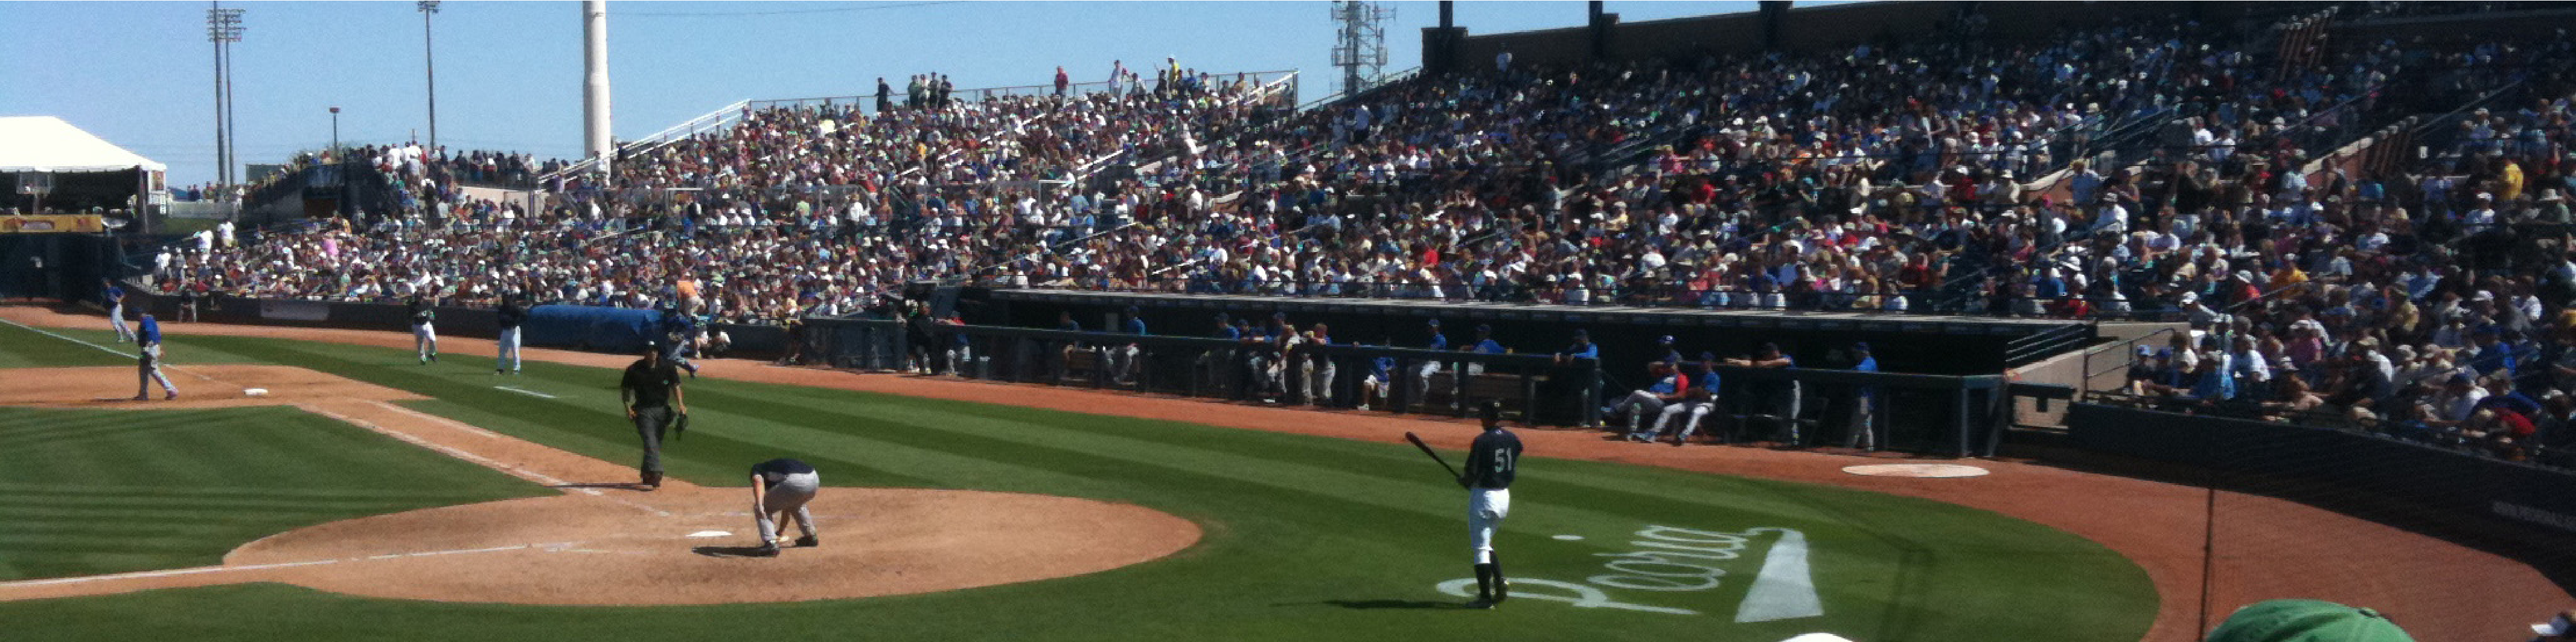
\includegraphics[height=1.5in]{images/sampleteaser}
%%   \caption{Spring Training 2009, Peoria, AZ.}
%% }

\maketitle

\begin{abstract}



\end{abstract}

\begin{CRcatlist}
  %\CRcat{I.3.3}{Computer Graphics}{Three-Dimensional Graphics and Realism}{Display Algorithms}
  %\CRcat{I.3.7}{Computer Graphics}{Three-Dimensional Graphics and Realism}{Radiosity};
\end{CRcatlist}

\keywordlist

%% Use this only if you're preparing a technical paper to be published in the 
%% ACM 'Transactions on Graphics' journal.

\TOGlinkslist

%% Required for all content. 

\copyrightspace

\section{Introduction}

All computer painting programs must store data through rasterization or vectorization. 
However, traditional computer painting programs take inputs of the same type as the stored data. The 
extremely popular Adobe programs Photoshop and Illustrator exemplify this. The former
allows a user to paint how he would on a physical medium. By letting the mouse act as
a brush, a user may color individual pixels on the screen. The latter lets a user paint
using geometric primitives such as lines and B\'{e}zier curves. The program then stores
these geometric primitives in order to render the drawing. Although using vector graphics
is likely less intuitive, it has some distinct advantages. First, there is no resolution
limit. One can zoom into an image as much as he would like and still see crisp edges.
Second, certain editing operations may be easier to perform on vector graphics.

In this paper we introduce TrianglePainter which  
uses a slightly different representation than traditional raster or vector graphics.
We instead use triangle meshes to store the data of the painting.
Since triangles are a geometric primitive used in vector graphics our approach achieves the
same advantages traditional vector graphics have. However, our representation allows the
user to paint with vector graphics without worrying about the underlying implementation.

In order to paint in our program the user simply drags his mouse on the screen to make
strokes akin to the process in a raster graphics program. Upon mouse-up the stroke is
converted to our underlying triangle mesh representation. In this way a user may paint using
vector graphics without worrying about the representation.

Furthermore, our representation allows painting at any scale. A user can make large strokes
while zoomed out and then zoom in to make fine details. All of this can happen without
loss of quality since the data is stored using triangles, not in pixels.

To do the transformation we use a combination of rasterization and marching squares to
determine the contour of the stroke. From the contour we can create a Delaunay triangulation
to represent the stroke. By then introducing a merging process we can take the triangulation
of the new stroke and combine it with the triangulation of the existing canvas. This yields
a new canvas with all the strokes combined.

TrianglePainter reduces the barriers in creating vector graphics. This in turn allows 
artists to focus on the painting and not the way in which they paint, while still 
getting the editing benefits of vector graphics.

\section{Related Works}

Previous work has focused on converting images into vector graphics to take advantage of the
efficient storage, easy editing, and infinite resolution it provides. For example \cite{lecot:ARD:2006}
minimizes an energy function to segment an image into a number of regions that are bounded
by cubic splines and filled with solid colors or gradients. A different approach by \cite{Lai:2009:ATG:1531326.1531391} 
automatically creates gradient meshes with support for holes. Yet another example is \cite{10.1109/TVCG.2012.76} 
which converts an image into a triangle mesh. All three of these can convert images into
a vector representation, yet none of them allow a user to create a painting in the vector medium.

Other work has proposed novel vector graphic data structures. For example \cite{Frisken:2000:ASD:344779.344899}
defines Adaptively Sampled Distance Fields (ADF). ADFs specify a signed distance function to a surface.
to render the shape requires sampling the function to determine whether or not a pixel is on the surface.
A quadtree accompanies the distance function to specify where higher sampling rates are necessary. \cite{Bremer:2001:VCM}
further describes how ADFs can be created and used. However, it is unclear how ADFs might be used in a general
painting program where strokes with solid colors and gradients are composited on top of one another.

Another series of works have created entirely new ways of painting. Diffusion curves as specified in \cite{Orzan:2008:DCV:1360612.1360691}
describe a new painting technique where the artists specify edges and colors for those edges. Their system
then solves a Poisson equation to diffuse the colors between boundary conditions specified at the edges.
The algorithm produces some truly beautiful drawing. Similarly \cite{McCann:2008:RGP:1360612.1360692}
lets artists paint in the gradient domain. Both of these approaches yield fantastic works of art, yet
they are really new mediums for artists to explore rather than a vectorized version of conventional
painting techniques.

Work has also been done in multi-resolution painting using raster graphics. \cite{Berman:1994:MPC:192161.192181}
stores image information in a quadtree so that different parts of the image can have different levels of detail.
This means the image effectively has an infinite level of detail, yet since it is stored in raster form
there are still limitations. For example a stroke painted at coarse detail will still look blurry when
zoomed in. The strokes are limited to the resolution they are painted at. \cite{Carr:2004:PD:1186562.1015809}
also allows the development of multi-resolution images using rasters, and as such suffers from the
same limitations. Another multi-resolution approach by \cite{Perlin:1995:LPP:218380.218437} uses
procedural textures to avoid any fundamental limit on resolution. Although useful for textures,
generating procedural textures is difficult and does not help artists easily create.

Our work builds on these findings. However, our goal is to enable artists to create vector
graphics through standard painting techniques without having to deal with the underlying representation.
We use the triangle mesh structure described in \cite{10.1109/TVCG.2012.76} to build a painting program
where the triangle mesh is created while the artists lays down strokes. 

\section{The Canvas Model}
The data necessary to render the painting resides in the canvas. However, the canvas contains more than just
a triangle mesh and understanding the underlying data structures is important for 
understanding the rest of the algorithm.

\subsection{Triangle Mesh}
When a user paints he generates points that are stored on the canvas. These points are
connected to form a triangle mesh. In every triangle the vertices are colored to either
produce a solid color or a linear gradient. In fact a given point that is part of
multiple triangles can take on different colors in each triangle. Note that although
the points are persistent, the triangles are not.

\subsection{Boundary Edges}
Although the triangles may change over time, they must abide by constraints known as
boundary edges. A boundary edge connects two points and specifies that no triangle
can cross it. Like points, boundary edges are persistent. So as triangles come and go they
may never cross a boundary edges.

\subsection{Results}


\begin{figure}
    \centering
        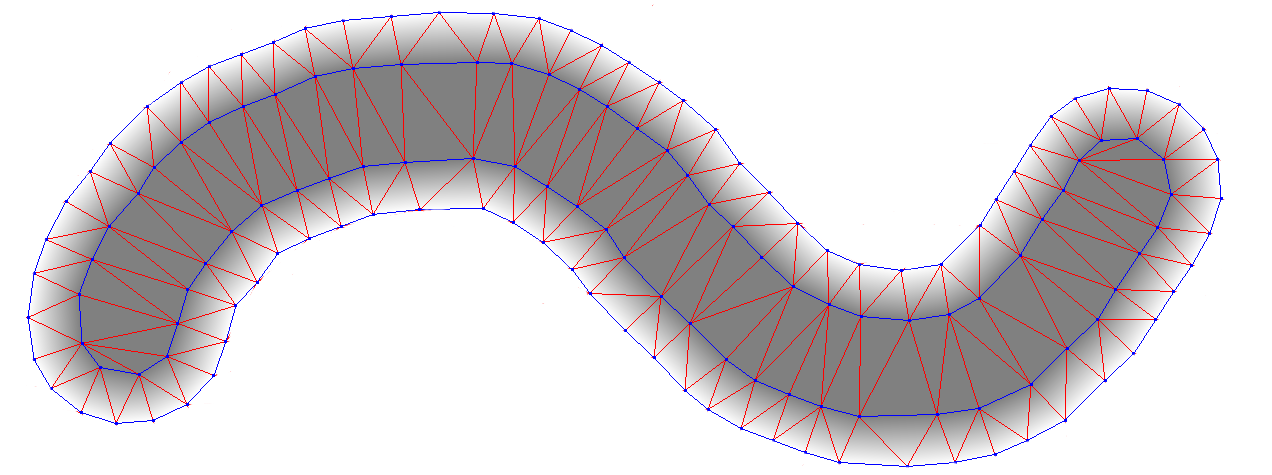
\includegraphics[width=0.4\textwidth]{images/stroke}
    \caption{An example triangulation. Blue lines are boundary edges. Black lines form the triangle
    mesh with the blue lines.}
\end{figure}

\subsection{Color Arcs}
Since triangles are not persistent they cannot store color data.
Storing colors in points works well when the color is the same for all triangles connected
to that point. However, when a point lies on a sharp boundary it may take on different colors in
triangles on either side of the boundary. The need for the same point to take on different
colors in different triangles lead to the development of color arcs.

A color arc has three components: a start vector, an end vector, and a color. 
Determining the color of a vertex in a given triangle requires two steps. First,
the vector from the point to the centroid of the triangle is calculated. Second,
the color arc is found which contains this vector. Containing the vector means one must turn
clockwise from the starting vector to reach it and counter-clockwise from the ending vector.
The point takes on the color of the arc in which the vector from the point to the centroid resides.

The color arcs for every point must satisfy three conditions. First, they must be disjoint. Second,
they must cover all $2\pi$ radians around the point. These first two conditions ensure that for any
triangle a point will take on exactly one color. Third, the start and end vectors must line up
with boundary edges. This condition makes all colors and gradients emanate from boundaries.

\begin{figure}
    \centering
        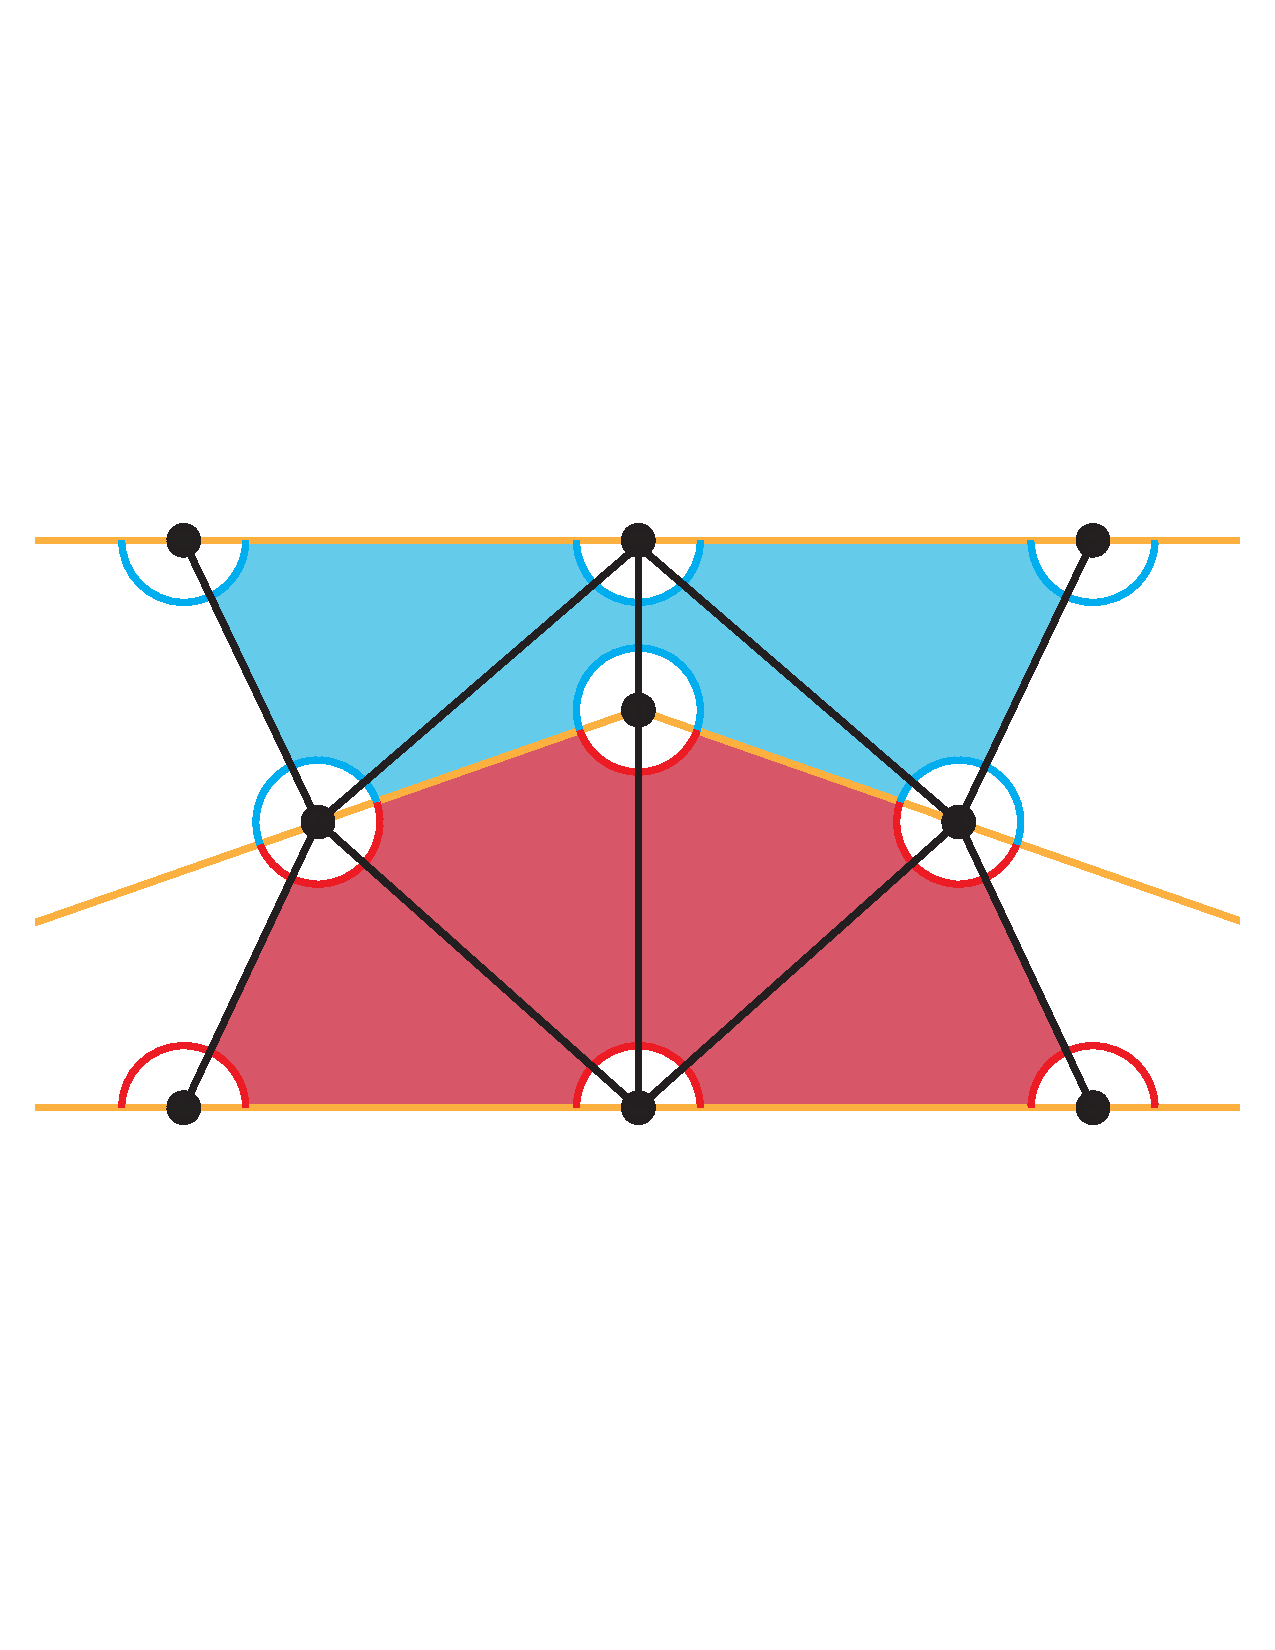
\includegraphics[width=0.4\textwidth]{images/colorarcs}
    \caption{An example of color arcs. The orange lines are boundary edges. Black lines form the triangle
    mesh with the boundary edges. Each point is given a color arc which defines its color in that range.
    Note that the points in the middle row have different colors on top and bottom. This gives blue
    triangles on top and red on bottom with a hard boundary in between.}
\end{figure}

\subsection{Rendering}
Once the triangle mesh has been generated it is simple to render. In each triangle the vertices
take on a given color based on their color arcs and the centroid of the triangle. If the three
vertices in the triangle take on the same color value then the triangle will be solid. If instead the 
vertices take on different color values then there will be a gradient over the triangle.

Since the conditions on color arcs make colors emanate from boundaries it's easy to create regions
containing either a solid color or linear gradient. A region will have a solid color if the
boundaries that surround it all take on the same color. If instead a region is surrounded by
two boundaries, one which has a given color and the other which has a transparent version of that color
then there will be a linear gradient in that region between the two boundaries.

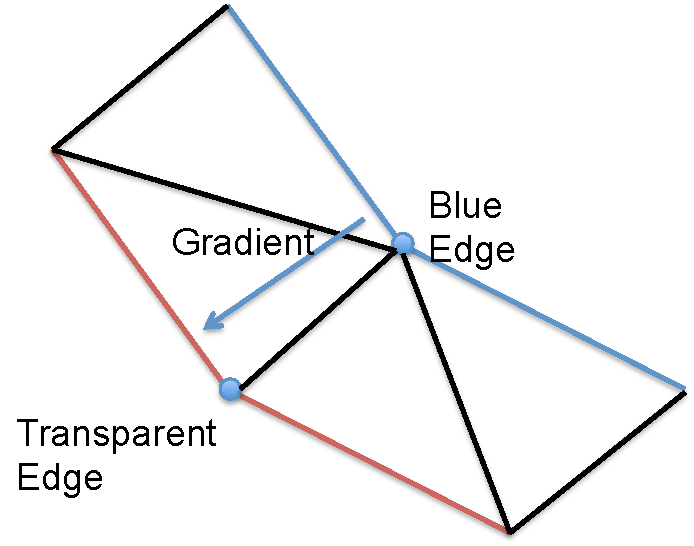
\includegraphics[height=1.5in]{images/softstrokeboundaryedges}


\section{Triangulating Strokes}

Here we consider how to convert a user's cursor motion into a triangle-mesh representation
of their stroke.

\subsection{Converting Strokes to Contours}
A set of contours define the outline of a stroke. For simply connected strokes, those without holes, 
one contour describes the whole stroke. However, strokes with holes, such as a circle or 
figure-eight, will have more than one contour.
Converting a user's mouse motion into a set of contours requires two steps.
First, the user's mouse movements are captured by a set of polygons which can be
rendered to yield a rasterized version of the stroke.
Second, to obtain the contours the stroke is rasterized in black and marching squares
is run to extract iso-contours of 50\% gray. This returns a very dense set of points 
which we reduce through a pruning process to
get a sparse but accurate representation of the contour.


Adam and Steve should we talk about how anti-aliasing + marching squares can achieve sub-pixel
resolution?

% Note that despite the reliance on rasterization it is still possible by using
% anti-aliasing and certain brushes to get sub-pixel resolution.

\subsection{Converting Contours to Triangles}
The contour contains two important pieces of information. First, it describes all of the points of the stroke.
Second, segments connecting adjacent points describe the boundaries of the stroke. 
A triangle mesh must contain all the points and stay
within the boundaries. For example, a concave contour should not contain triangles inside the concavity since such triangles
would be outside of the boundary.
Furthermore, these boundaries will later be crucial when compositing a stroke onto a canvas.

We utilized Jonathan Shewchuk's Triangle library to perform Delaunay triangulations
on the given set of points and boundaries. The library outputs a mesh that
approximately represents the drawn stroke.

\begin{figure*}
\centering
\begin{subfigure}[b]{0.3\textwidth}
  \centering
  
\includegraphics[width=.9\textwidth]{images/stroke_triangulation/hardrendered}
  \caption{A subfigure}
  \label{fig:sub1}
\end{subfigure}%
\begin{subfigure}[b]{0.3\textwidth}
  \centering
  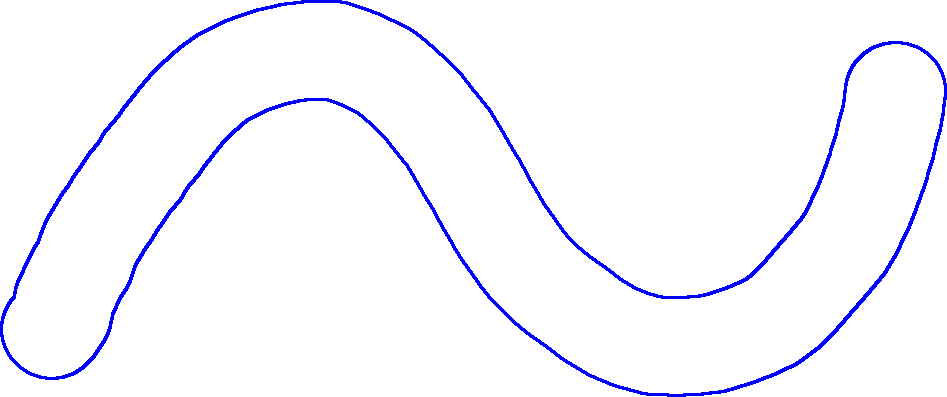
\includegraphics[width=.9\textwidth]{images/stroke_triangulation/hardpruned}
  \caption{A subfigure}
  \label{fig:sub2}
\end{subfigure}
\begin{subfigure}[b]{0.3\textwidth}
  \centering
  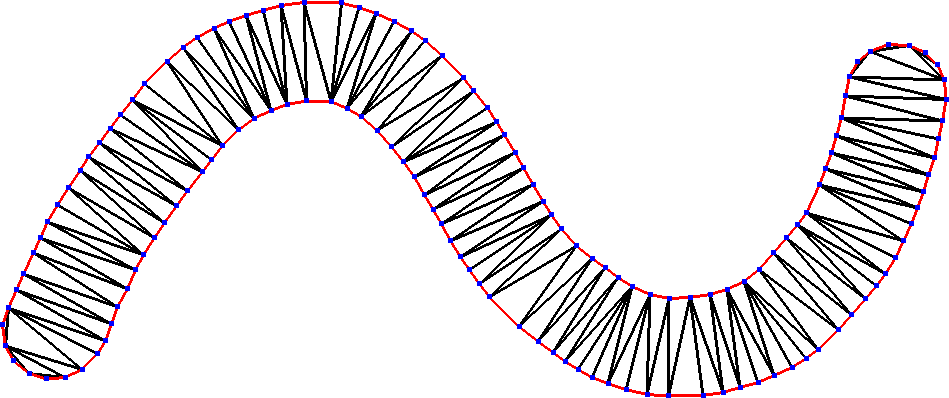
\includegraphics[width=.9\textwidth]{images/stroke_triangulation/hardmesh}
  \caption{A subfigure}
  \label{fig:sub2}
\end{subfigure}
\caption{A figure with two subfigures}
\label{fig:test}
\end{figure*}

\begin{figure*}
\centering
\begin{subfigure}[b]{0.3\textwidth}
  \centering
  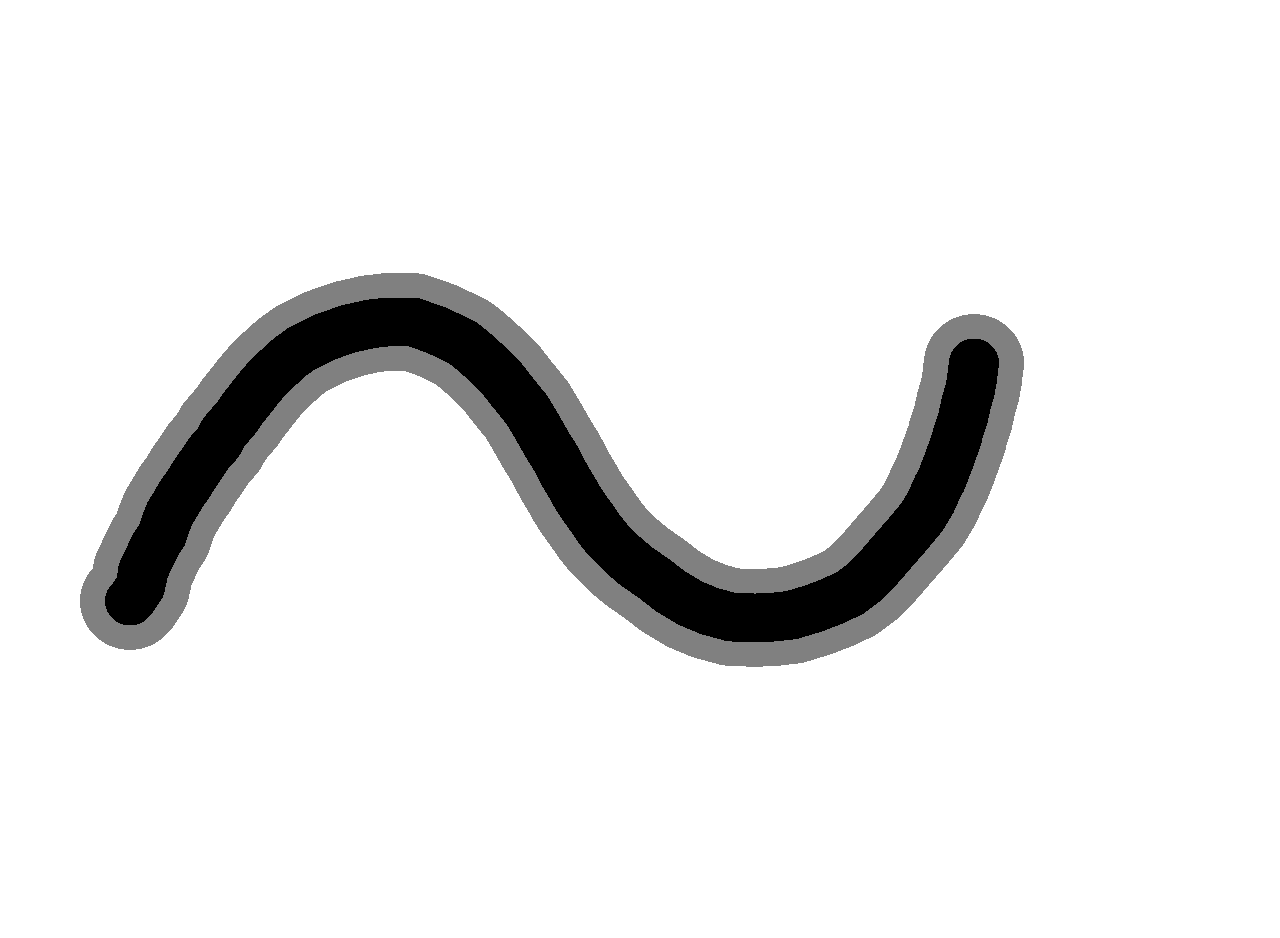
\includegraphics[width=.9\textwidth]{images/stroke_triangulation/softrendered}
  \caption{A subfigure}
  \label{fig:sub1}
\end{subfigure}%
\begin{subfigure}[b]{0.3\textwidth}
  \centering
  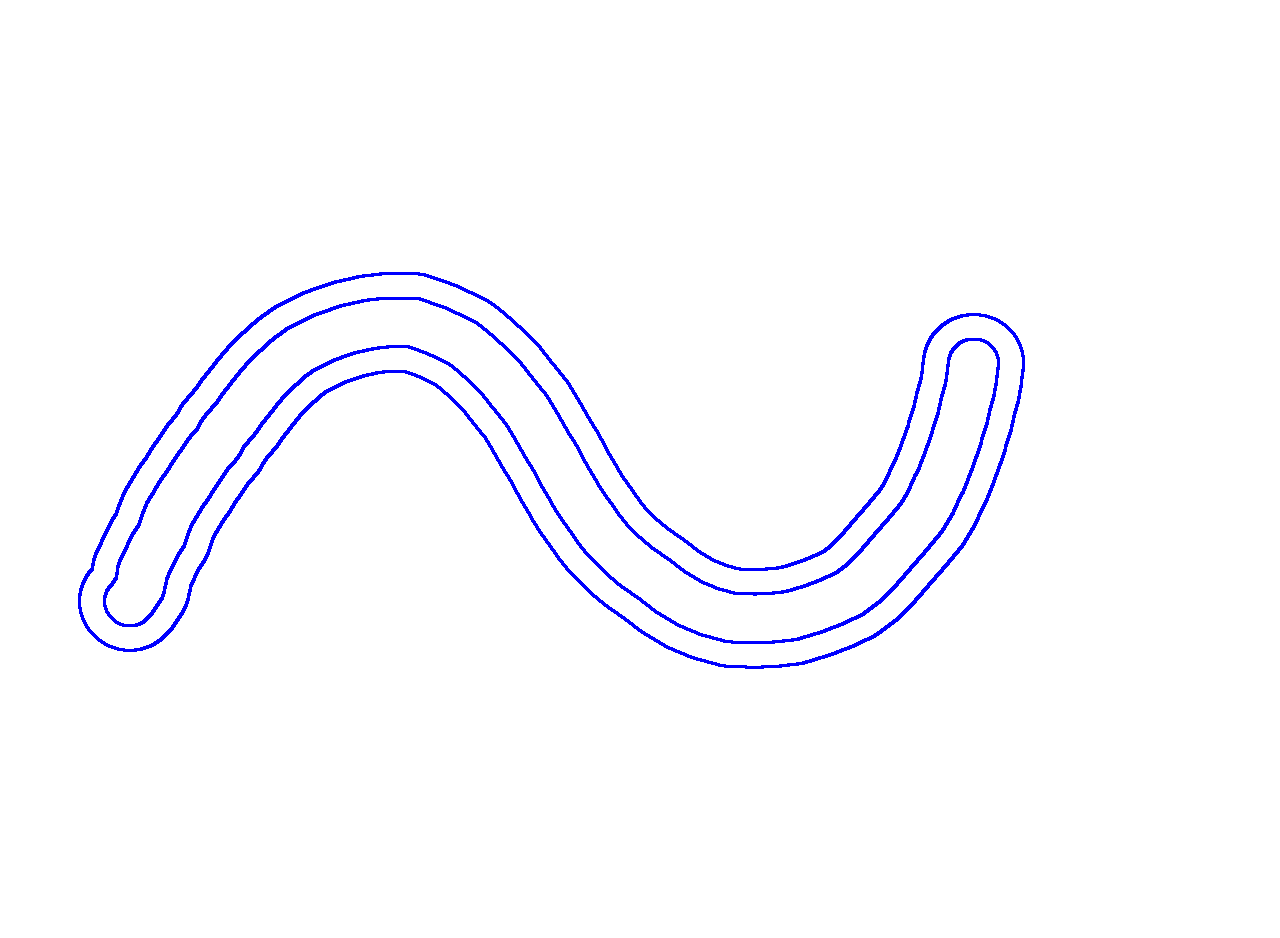
\includegraphics[width=.9\textwidth]{images/stroke_triangulation/softpruned}
  \caption{A subfigure}
  \label{fig:sub2}
\end{subfigure}
\begin{subfigure}[b]{0.3\textwidth}
  \centering
  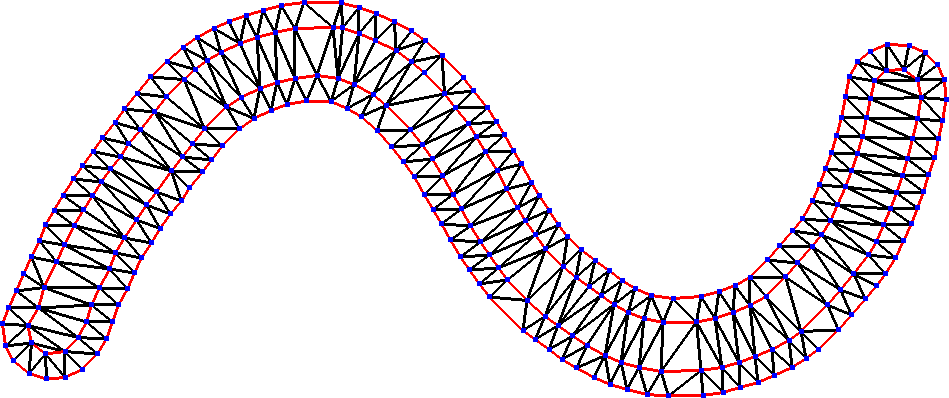
\includegraphics[width=.9\textwidth]{images/stroke_triangulation/softmesh}
  \caption{A subfigure}
  \label{fig:sub2}
\end{subfigure}
\caption{A figure with two subfigures}
\label{fig:test}
\end{figure*}


% 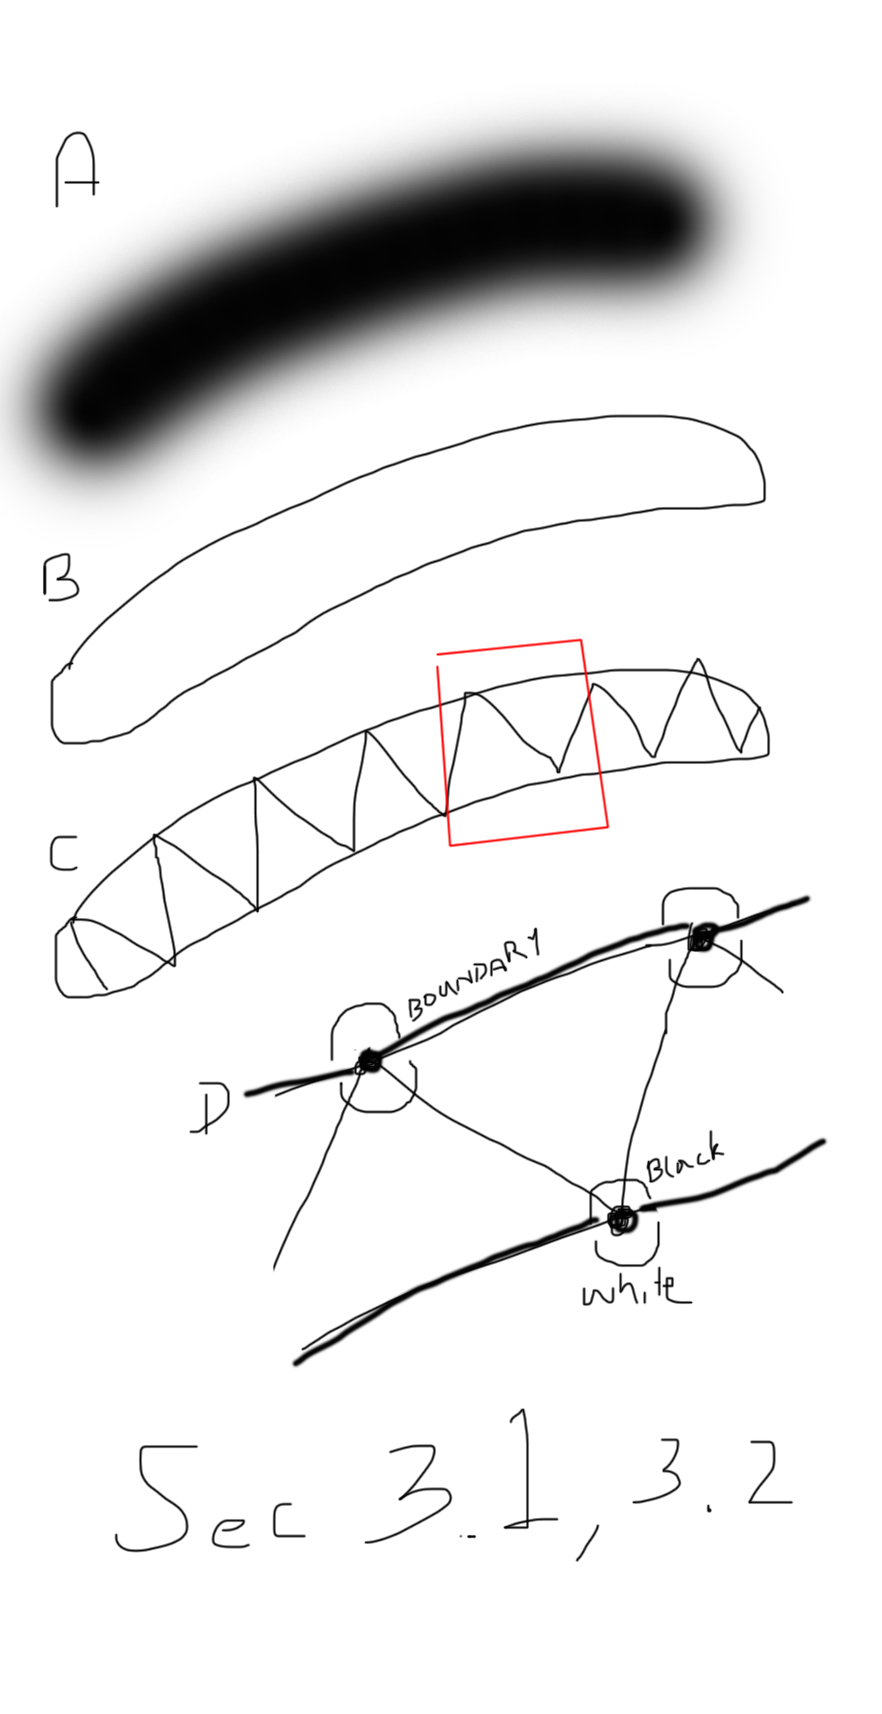
\includegraphics[height=1.5in]{images/triangulationprocess}

\subsection{Soft Strokes}
The above procedure converts a hard brush into a triangle mesh. Yet, a somewhat more interesting
case is converting a soft brush with linear gradient into a triangle mesh. A soft stroke has two
components, an inner hard stroke and an outer gradient stroke. Since the triangles in the inner and
outer parts of the stroke must be colored differently, none of the triangles may cross the boundary
between the hard and soft regions.

This representation needs a slightly different procedure. The user's mouse motion
is capture in two sets of polygons. The first set describes the outer soft stroke and the second set describes
the inner hard stroke. Next the outer stroke polygons are rendered in 50\% gray and the inner stroke
is rendered in black. This means the boundary of the outer stroke is the 25\% gray iso-contour and the
boundary of the inner stroke is the 75\% gray iso-contour.

Again, using marching squares these contours are extracted and then pruned. The boundaries and points
derived from the contours are fed into Triangle and a mesh is returned. This mesh represents the soft
stroke where no triangle crosses the boundary between the soft and hard parts
of the stroke.

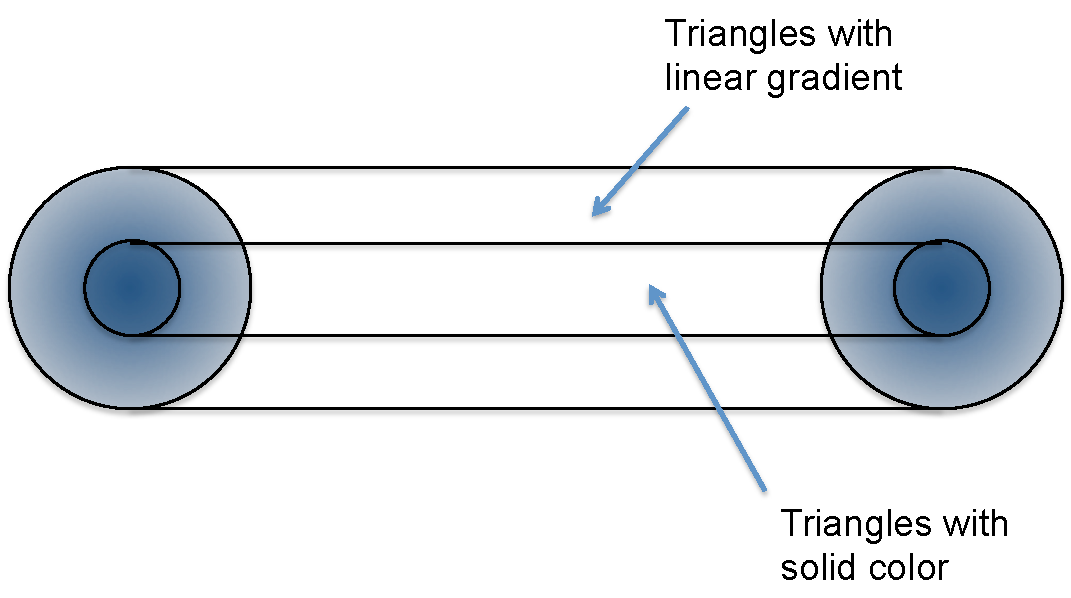
\includegraphics[height=1.5in]{images/softstroke}
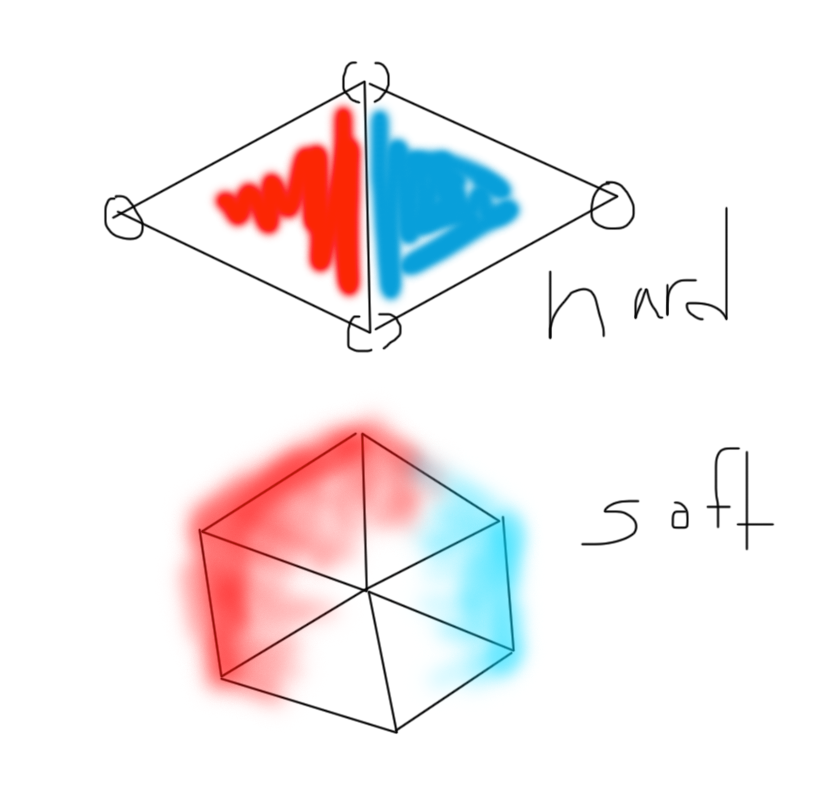
\includegraphics[height=1.5in]{images/hardvssoft}

\section{Compositing Strokes}
Once the stroke has been converted to triangles by the above procedure it is necessary to
composite the stroke onto the canvas. We first consider the canvas model and then how a
stroke can be composited onto the canvas.






\subsection{Adding Points to the Canvas}

Every canvas begins with four points, one at each corner of the screen, and four boundaries, one
for each edge of the screen. These points are originally part of two big triangles which
divide the canvas.

In the simplest approach the points and boundaries from the new stroke are added
to the list of points and boundaries already stored. All of this data can be fed into Triangle
to produce a new mesh. The new mesh contains all of the points of the old and new strokes. Since
all of the boundaries are stored and fed into Triangle the stroke edges are preserved. This means that
no triangle can cross the boundary of a stroke. Without this constraint it would be impossible to color the
triangles since they would straddle color arcs. Once a new mesh is formed the color arcs of the 
new and old points must be computed.

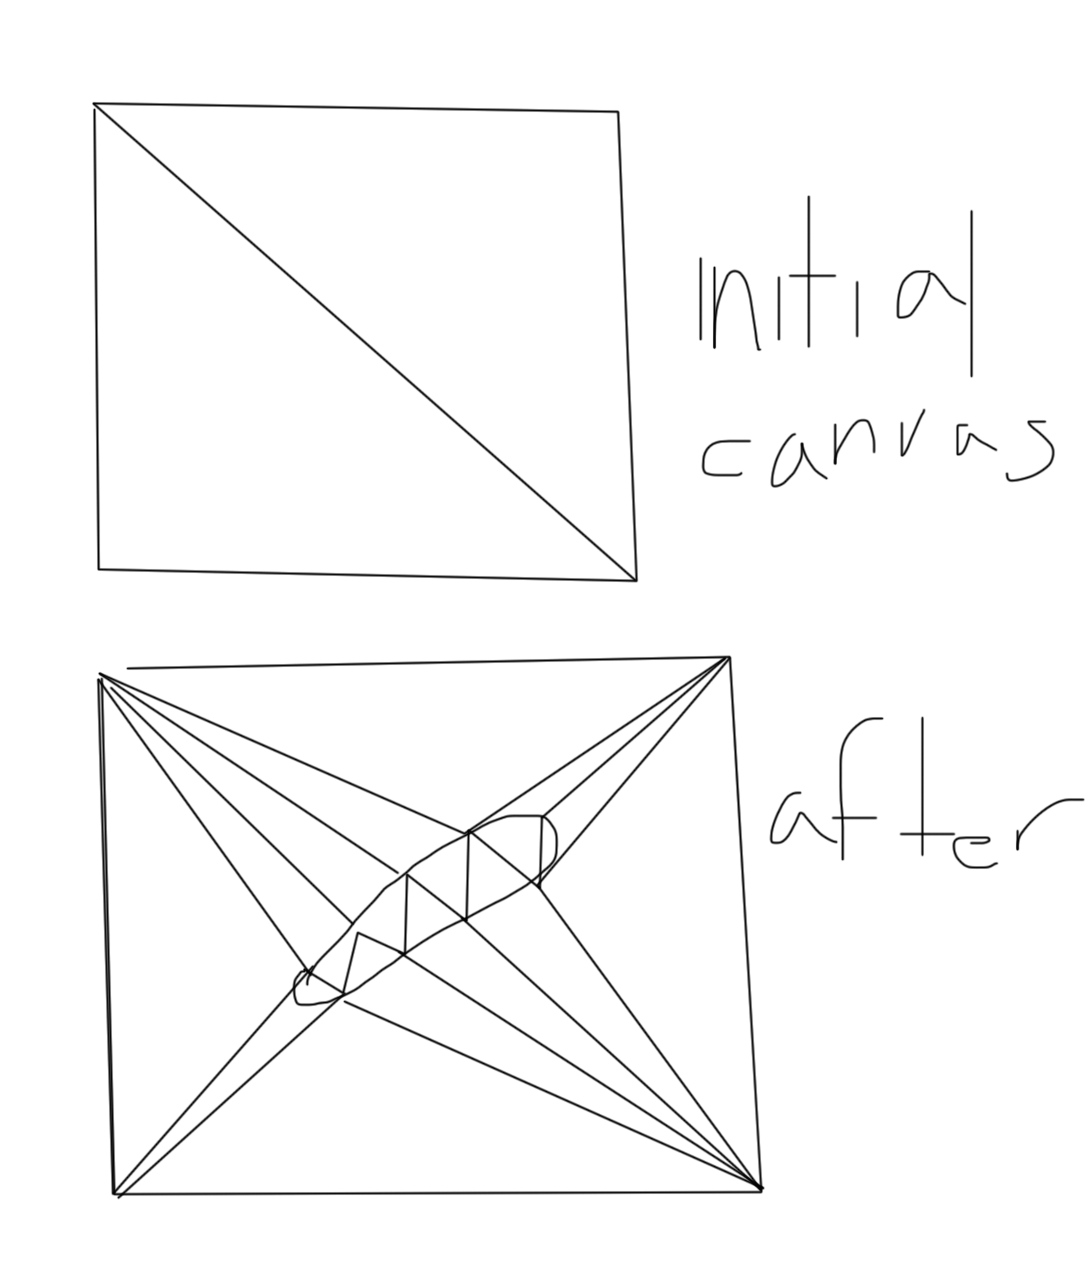
\includegraphics[height=1.5in]{images/canvastriangulation}

\subsection{Determining Colors}
The color arcs for new points depend on two values, the color of the stroke and the color
of the canvas at that point. The points on a hard stroke will have two color arcs. One
arc describes the inside of the stroke. The color for this arc is the color of the stroke
composited over the color of the canvas at that point. The other arc describes the outside
of the stroke. The color for this arc is just the color of the canvas at that point. The
points on a soft stroke will have one color arc. The color arc for points on the inner
contour is the color of the stroke composited over the color of the canvas at that point.
The color arc for points on the outer contour is the color of canvas at that point.
This gives any triangle connecting inside and outside contour points a linear gradient
from the stroke color composited over the canvas color to the canvas color.

The color arcs for old points remain the same unless part of the new stroke covers it.
In this case the colors in each arc must be replaced with the stroke color composited over
the old color of the arc. If the new stroke is soft then the color at the location of
the old point must be determined through bilinear interpolation before compositing.




\subsection{Intersection Points}

When Triangle is asked to triangulate a set of points with overlapping boundaries it must
insert a point at the intersection, since without it at least one triangle would have to
cross a boundary. These points are introduced with no color information, but the final colors for 
all of the other points in the mesh have already been determined.

An intersection point lies on two boundaries and therefore has four boundary edges emanating from it. 
To determine the colors of an intersection points requires knowing the colors associated with
points on the boundaries. For both boundaries travel both directions to the first point with color data. Note this may not
be the first point on each side since this intersection point may be adjacent to other intersection
points without color data. For both boundaries linearly interpolate the colors in the color arcs. 
This yields four average colors, two from the new stroke boundary and two from the old stroke boundary.
The colors from the new stroke are composited over the colors from the old stroke to yield four new
colors, one for each region defined by the boundary intersections. 

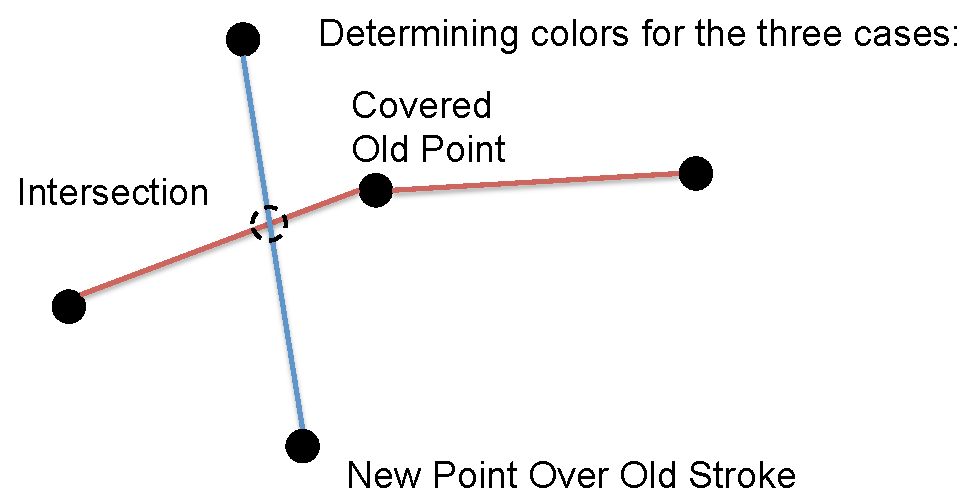
\includegraphics[height=1.5in]{images/determiningcolors}

\subsection{Finding Modified Points}
The above procedure has two important drawbacks. First, it processes many points that don't need
consideration which takes a considerable amount of processing time. Second, since it acts on the whole
canvas, local changes can have global effects. To avoid this problem the algorithm determines
which triangles can remain
and which triangles need to be included in the re-triangulation. To accomplish this a static grid
is generated and all of the cells which contain a triangle from the new stroke are marked. 
The set of triangles from the old triangulation that intersect these grid squares are found.
The set of edges from these triangles that do not intersect these grid cells form a ring
around the area of our new triangles. The edges in this ring become constraints
in the triangulation. All of the points and constraint edges from the old triangulation are
included as well as the points and constraint edges from the new triangulation. Triangulating
these points and edges gives the new geometry for the modified area and has no effect on any
other part of the canvas. Therefore, the old triangles from the rest of the canvas can be reused. 
The new triangulation combined with the old triangles give a new triangle mesh representation of the entire canvas.

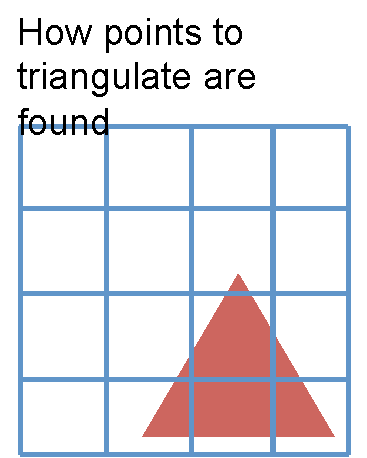
\includegraphics[height=1.5in]{images/findingmodifiedpoints}

\section{Discussion and Results}
Our work with this algorithm has lead to observations in three main areas.

\subsection{Stability}
Something we've worked hard to achieve is program stability. Certain geometries are fatal
for the Triangle library. The current instability in the program is normally caused by
providing the library with such difficult geometries. To improve program stability would
require addressing geometries such as vertices that are too close together. This would
take more processing time and is something we have yet to explore. However, clearly this
problem must be solved before the program could be used formally.

\subsection{Performance}
The current implementation uses Python and PyOpenGL. Python's performance is slower than
a lower level implementation in C++ would be. The drawing of the canvas is quick with
no lag. However, the actual process to extract a stroke from rasterization to triangle
representation on the canvas is slow. On a blank canvas strokes take on the order of
1 second to process. However, on a canvas with lots of geometry a stroke that covers
that geometry can take several seconds to render. Some of this time is due to poor
implementation of the algorithm. However, there are lots of calculations
to do with the old points affected by the new stroke and the points associated with the
new stroke itself. Since these geometries can get arbitrarily complicated, these
calculations can take an arbitrarily long. This brings us to the final point, scalability.

\subsection{Scalability}
No matter how good the implementation, the fact that paintings can get arbitrarily complicated
means there must be some way to simplify the mesh. Although we have yet to implement
such a simplification algorithm, we have a couple suggestions on how it might be done. In most situations where
a lot of strokes are composited on top of one another, most of the geometry is redundant. 
For example, when an opaque stroke is laid down on top of a complex geometry, that complex
geometry no longer has any useful information since the outline of the opaque stroke
completely defines it. Furthermore, even with translucent or feathered strokes, enough
composited strokes may produce complex geometry that does not add much to the output.
Some of this geometry can be reduced without noticeable changes in the output. Such a
simplification algorithm must be implemented to ensure a painter can continue to paint
without the program slowing to an unusable state.

\subsection{Complexity}
We now examine the growth of triangles, points, and boundaries on the canvas.


% \begin{tabular}{| l | l | l | l|}
%   \hline                       
%   Number of Strokes & Triangles & Points & Boundaries \\
%   \hline                       
%   1 & 360 & 229 & 229 \\
%   2 & 506 & 302 & 310 \\
%   3 & 652 & 375 & 403 \\
%   4 & 798 & 448 & 488 \\
%   5 & 972 & 535 & 603 \\
%   6 & 1164 & 631 & 713 \\
%   \hline  
% \end{tabular}
% 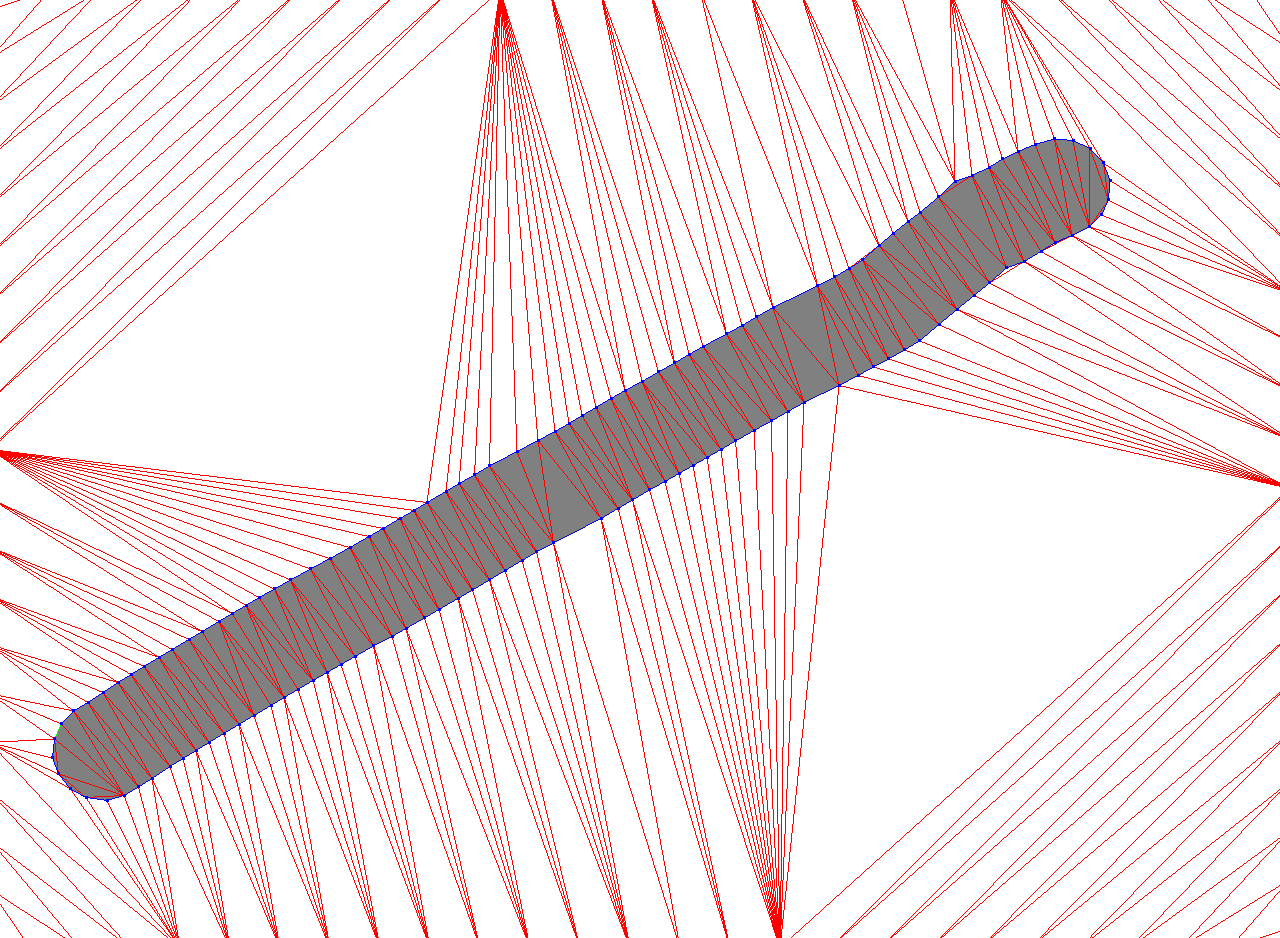
\includegraphics[height=1.5in]{images/tri360points229edges229}
% 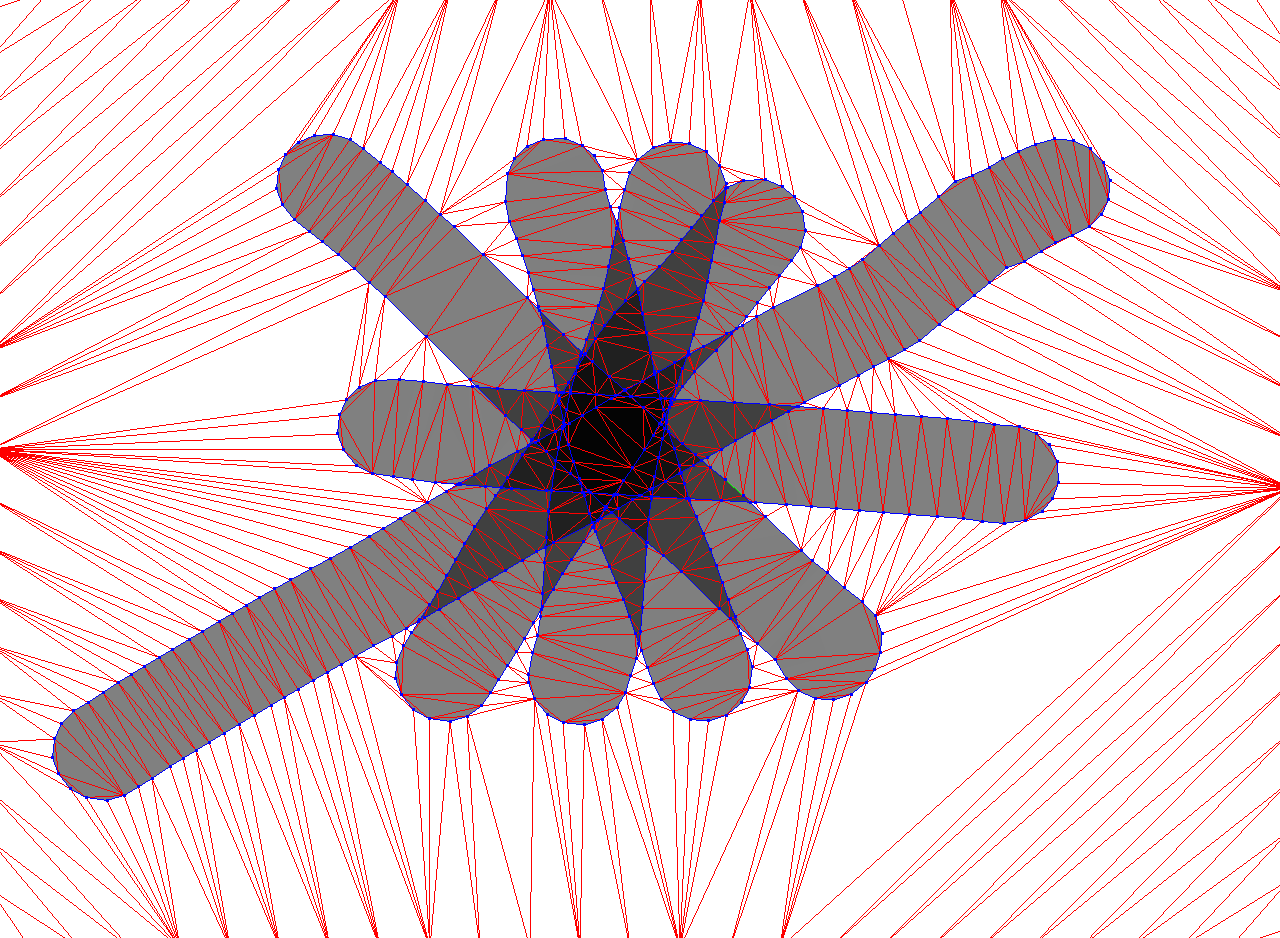
\includegraphics[height=1.5in]{images/tri1164points631edges713}

The complexity of the triangles increase slightly more than linearly since extra points and 
boundaries are made when boundaries intersect.

NOTES: 

-Maybe do the same analysis with soft strokes

-Look at the time it takes to render these strokes

-Then show more robust drawings and the number of triangles, points, and boundaries




\section{Conclusion}

\section*{Acknowledgements}

\bibliographystyle{acmsiggraph}
\bibliography{template}
\end{document}
